\documentclass[aspectratio=43, usepdftitle=false, xcolor={dvipsnames}]{beamer}
%infos
\usetheme[english, secslide, subsecslide, coloraccent=blue]{awesome}
\title{Comment optimiser ses chances de gagner une compétition de parkour ?}
\author[Elowan]{Elowan Harnisch}
\subtitle{To illustrate this awesome theme}
\institute{Institute of Software Engineering and\\Programming Languages}
\date{\today}
\background{images/background.png}

\begin{document}

\maketitle

% 1
\begin{frame}
	\begin{block}{Parkour/Freerunning}
	Le parkour (ou art du déplacement ou freerunning) est une discipline sportive acrobatique qui consiste à franchir des obstacles urbains ou naturels, par des mouvements rapides et agiles. Les pratiquants sont dénommés "traceurs" (Wikipédia)
	\end{block}

	\begin{block}{Compétition de parkour (Freestyle)}
	Compétition où des traceurs disposent d'une estrade avec du mobiliers pour faire des enchainements de figures. Le but étant d'avoir le plus de points, rapportés par ces dites figures, pour gagner.
	\end{block}

	\begin{figure}
		\center
		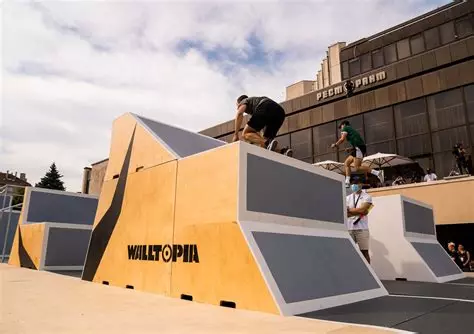
\includegraphics[width=0.35\textwidth]{images/terrain.png}
		©\url{https://walltopia.com}
	\end{figure}
\end{frame}


% 2
\begin{frame}{Représenter la réalité}
	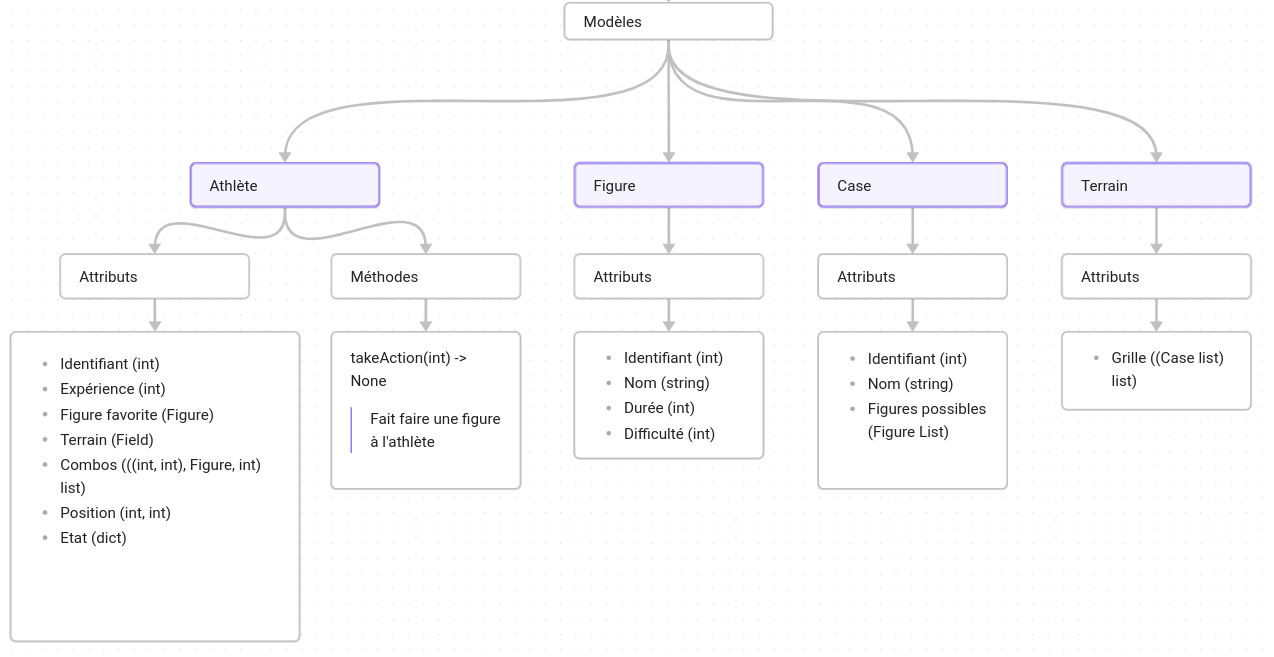
\includegraphics[width=1\textwidth]{images/modeles.png}
\end{frame}

\begin{frame}{Résoudre le problème}
	Utilisation d'un algorithme génétique pour trouver la solution optimale.
	\begin{figure}
		\center
		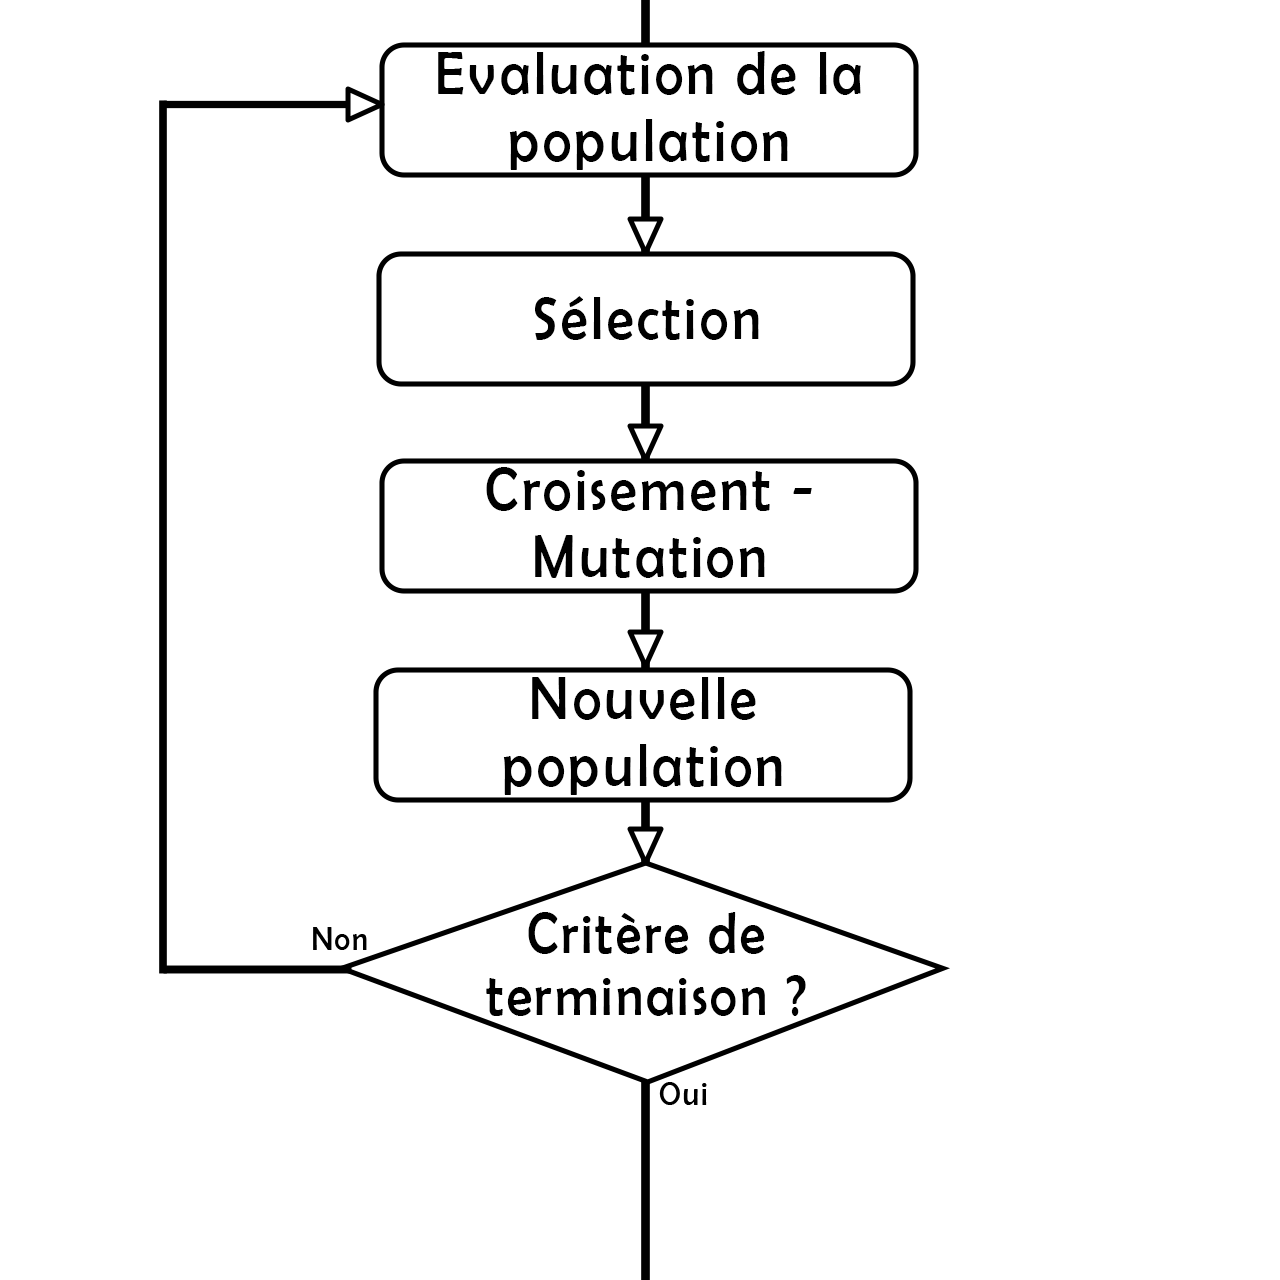
\includegraphics[width=0.6\textwidth]{images/Algo Genetq.png}
	\end{figure}
\end{frame}

% 3
% \begin{frame}{Premiers résultats et premiers problèmes}
% 	\includegraphics[width=1\textwidth]{images/first.png}
% \end{frame}

% 4
\begin{frame}{Athlète de $<$3, Lilou Ruel}
	\begin{figure}
		\center
		
\includegraphics[width=0.3\textwidth]{images/lilou.jpg}
		\caption{Lilou Ruel, championne du monde de Parkour/Freerunning (©\url{https://thehandbook.com})}
	\end{figure}
\end{frame}

\begin{frame}{Mise à l'épreuve}
	Lilou Ruel VS l'ordinateur
	
	\begin{figure}
		\center
		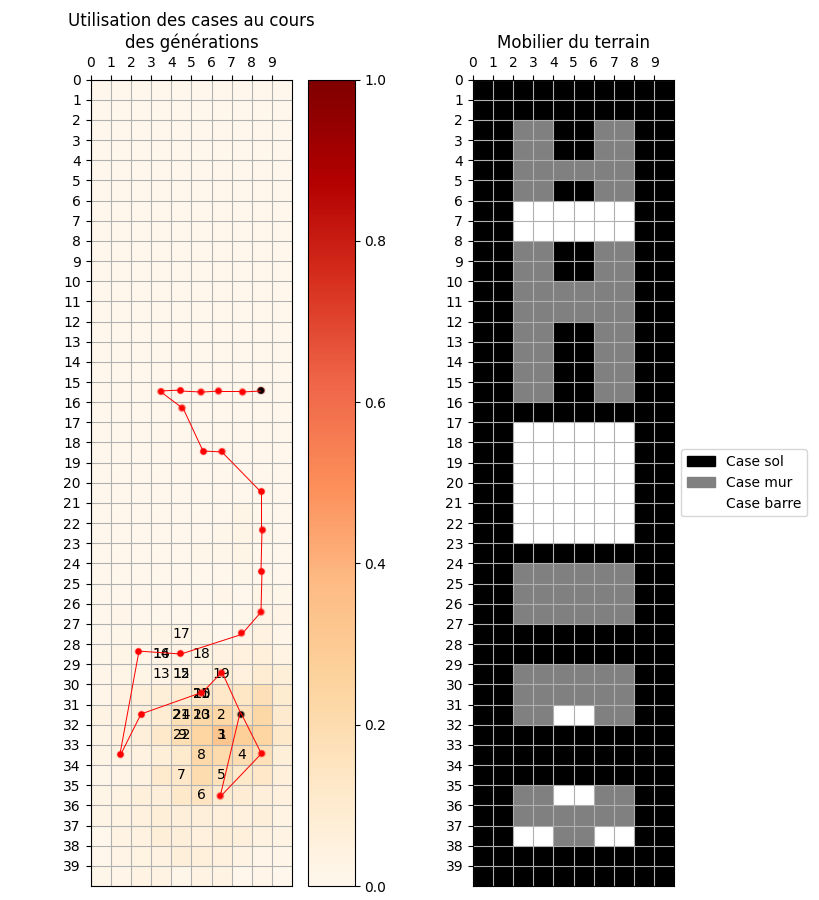
\includegraphics[width=0.6\textwidth]{images/LILOUcases.png} 
	\end{figure}
\end{frame}

\begin{frame}{Mise à l'épreuve}
	
	\begin{block}{Résultats de Lilou}
		\itemize{
			\item Score réel (Compétition à Sofia, Bulgarie) : 21
			\item Score obtenu par l'ordinateur (après reproduction de son parcours): 17.8
			\item Score moyen obtenu après algorithme génétique : 22.8
		}
	\end{block}

	\begin{figure}
		\center
		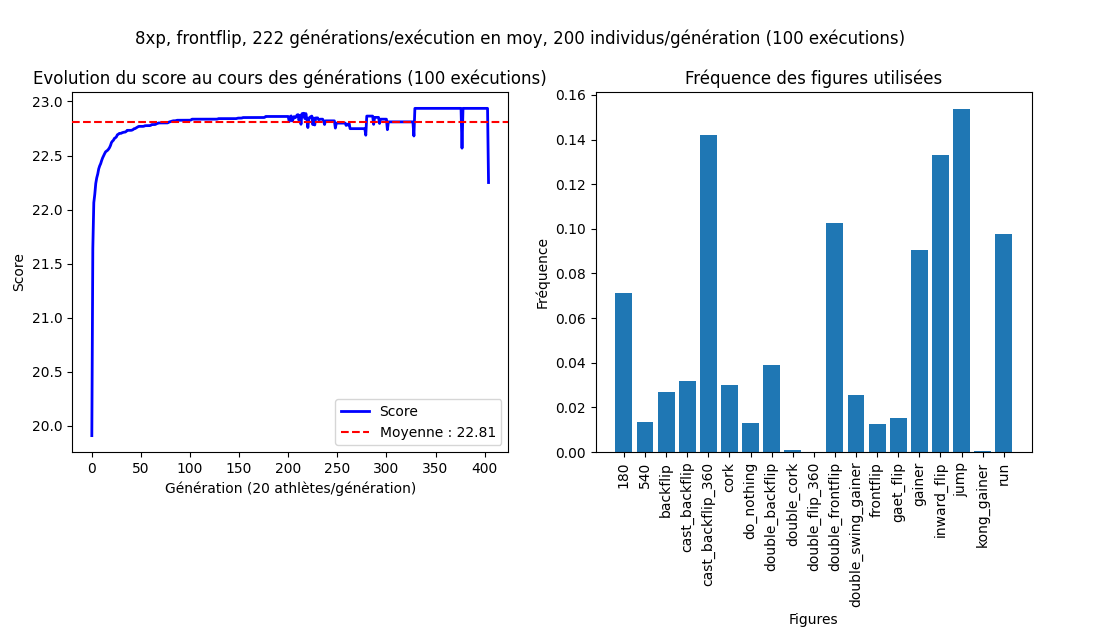
\includegraphics[width=0.9\textwidth]{images/LILOUfreq&fitness.png} 
	\end{figure}
\end{frame}

% 5
\begin{frame}{Pourquoi ça ne colle pas?}
	\itemize{
		\item L'athlète a fait des figures qui ne sont pas répertoriées
		\item La récupération de son parcours pose quelques problèmes
		\item Le remplacement de toute la partie humaine du jugement par de l'aléatoire
	}

\end{frame}

\begin{frame}{La conclusion}
	Tout n'est pas à jeter ! L'algorithme utilise bien les mêmes mécanismes que l'humain

	\begin{figure}
		\center
		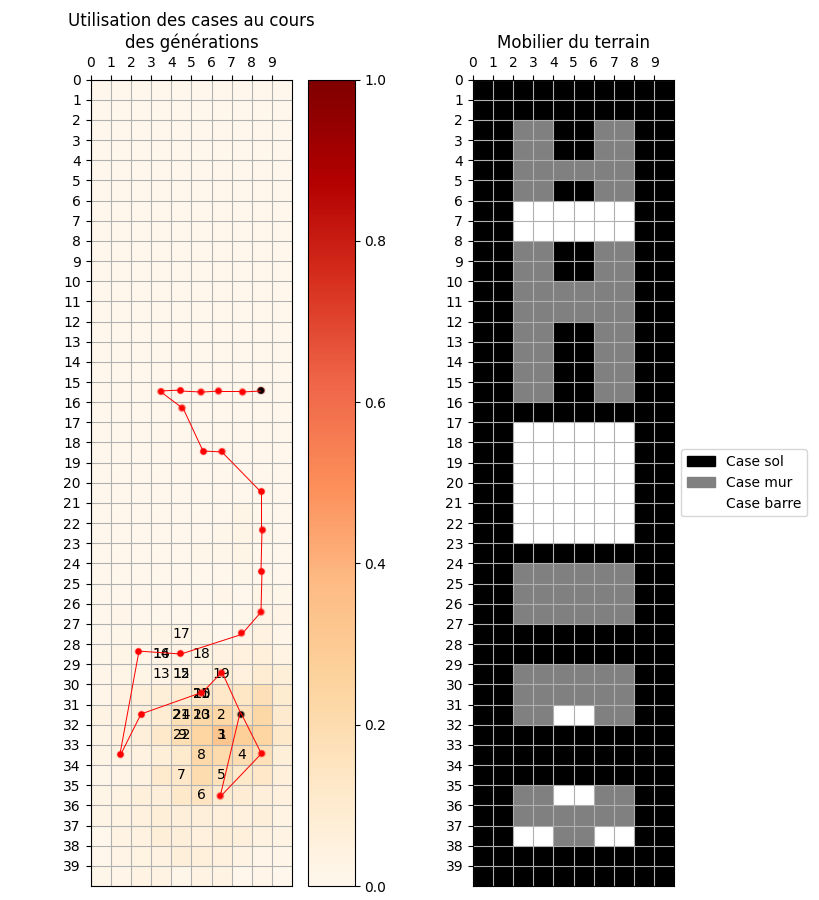
\includegraphics[width=0.55\textwidth]{images/LILOUcases.png} 
	\end{figure}
\end{frame}

\begin{frame}{Bibliographie}
	\begin{enumerate}[label={[\arabic*]}, noitemsep]
		\item [1] Sean Moriarity \textbf{Genetic Algorithms in Elixir}
		\item [2] Randy L. Haupt, Sue Ellen Haupt \textbf{Practical Genetic Algorithms}
		\item [3] FIG \textbf{PK Code of points 2022-2024 - Table of ticks 2023}
		\item [4] FIG \textbf{Code de pointage 2019-2021}
	\end{enumerate}
\end{frame}
 
\end{document}
